\section{测试环境、数据与评价指标}

本次测试使用的数据集规模、用途与核心评价指标如表 7 所示。实验主要使用 524 张验证集样本进行医疗主线评估，另使用 8 条金融边界压力样本进行迁移性与稳定性验证。医疗主线采用阈值精度、AUC 和 argmax 精度作为主要指标，其中阈值精度用于反映部署口径下的最终分类效果，AUC 用于衡量整体判别能力，argmax 精度用于描述未校准条件下的直接决策表现。协议层与控制面验证则采用异常输入拦截率、重放拦截率、并发守卫结果和审计落盘状态作为主要观察指标。

需要说明的是，本文中涉及的性能结果均以固定 checkpoint 和同口径验证集为基础，反映的是部署态结果而非多随机种子的训练均值。

\begin{longtable}{>{\raggedright\arraybackslash}p{0.24\textwidth}>{\raggedright\arraybackslash}p{0.24\textwidth}>{\raggedright\arraybackslash}p{0.24\textwidth}>{\raggedright\arraybackslash}p{0.24\textwidth}}
\caption{表 7 测试数据集与评价指标说明}\\
\toprule
\textbf{对象} & \textbf{样本规模} & \textbf{作用} & \textbf{主要指标} \\
\midrule
\endfirsthead
\toprule
\textbf{对象} & \textbf{样本规模} & \textbf{作用} & \textbf{主要指标} \\
\midrule
\endhead
医疗全量验证集 & 524 张 & 正式阈值搜索与精度评估 & argmax 精度、阈值精度、部署阈值 \\
医疗部署验证批次 & 32 张 & 完整双向隐私原型运行 & 平均时延、双向总通信量、隐私边界 \\
金融边界压力样本 & 8 条 & 极端分布输入下的稳定性验证 & 逐样本一致性、时延、通信量 \\
协议层与控制面黑盒用例 & 17 类 & 异常输入、重放与并发探针验证 & 首个拦截层、兜底层级、资源状态 \\
\bottomrule
\end{longtable}

\section{基线对比}

\begin{figure}[htbp]
\centering
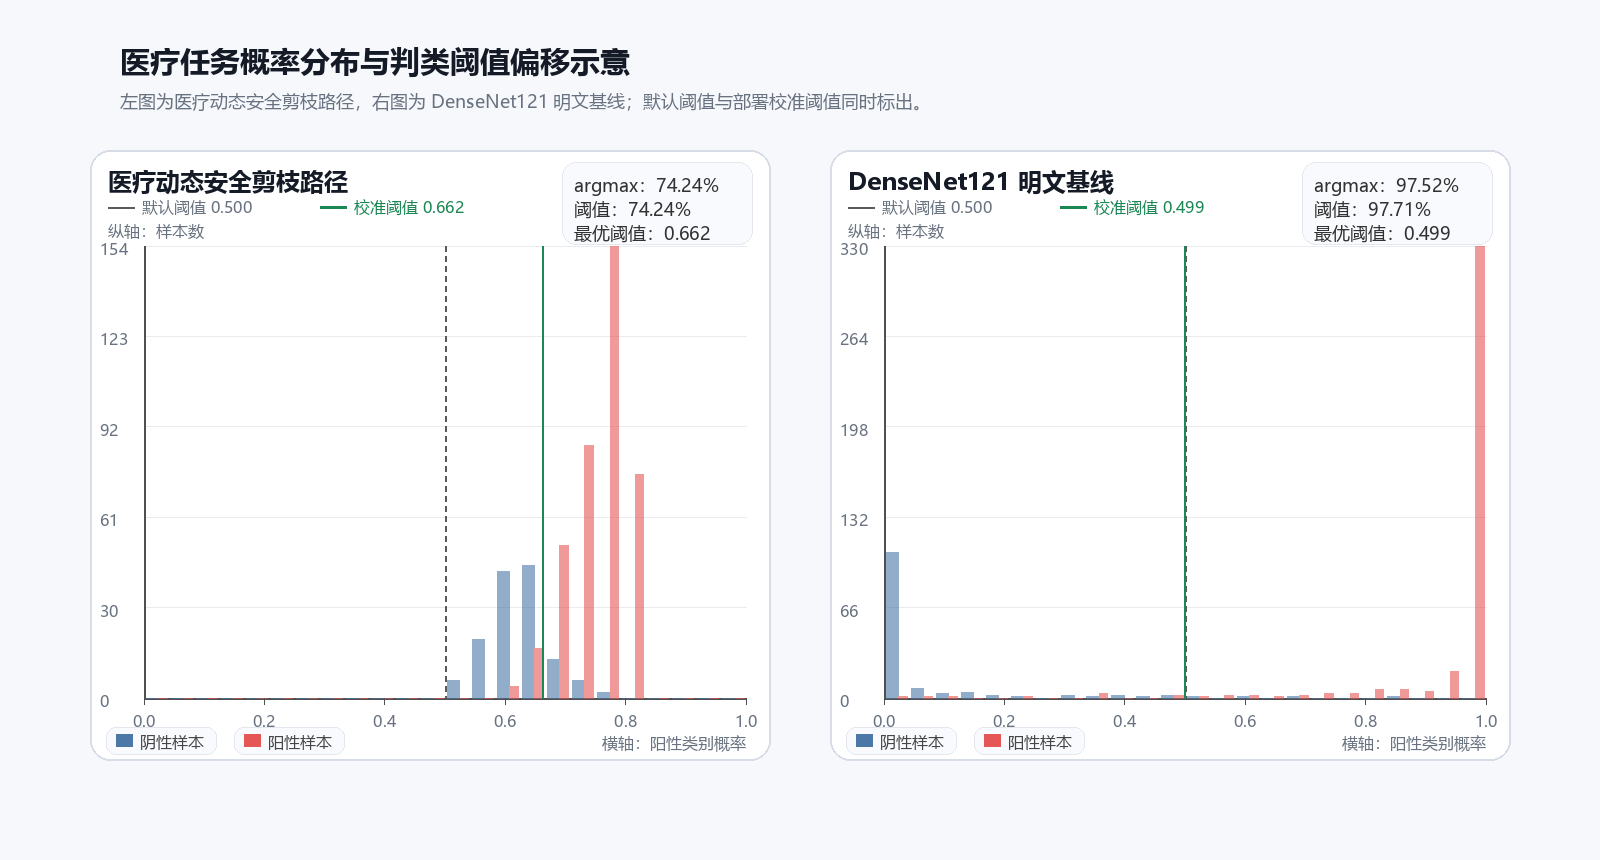
\includegraphics[width=0.92\textwidth]{figures/fig4-1-threshold-shift.png}
\caption{图4-1 不同方案医疗任务性能基线对比}
\end{figure}

本作品与不同基线方案在医疗任务上的性能对比结果如图4-1 所示。从同仓与外部对比结果看，本作品医疗动态安全剪枝链路相较固定结构静态对照线提升 0.7634 个百分点，相较当前仓内可复现的原始 DynamicViT 基线提升 17.3664 个百分点，说明协议友好重写并未使动态路径退化为不可部署状态。另一方面，与同数据集强明文参考 MPCViT（面向多方计算的视觉 Transformer）相比，本作品当前仍存在 4.2366 个百分点的阈值精度差距；与同架构静态上界 DeiT-S（数据高效图像 Transformer 小型模型）相比，差距为 3.2419 个百分点。这些差距说明本作品的价值主要在于“双向隐私 + 动态剪枝安全执行”的系统能力，而不是在明文精度指标上全面超过所有强明文参考。

需要说明的是，外部对比表中“原始 DynamicViT”一行现统一采用当前仓内与服务器均可复现的原始明文基线口径。此前遗留的“20 epoch / 80.73\%”旧值未能在最终交付仓与服务器环境中追溯到配套权重文件，因此本次修订不再继续引用该旧数值。

\section{医疗主要交付场景结果}

\begin{longtable}{>{\raggedright\arraybackslash}p{0.32\textwidth}>{\raggedright\arraybackslash}p{0.32\textwidth}>{\raggedright\arraybackslash}p{0.32\textwidth}}
\caption{表 8 医疗主要交付场景核心指标结果}\\
\toprule
\textbf{指标} & \textbf{结果} & \textbf{说明} \\
\midrule
\endfirsthead
\toprule
\textbf{指标} & \textbf{结果} & \textbf{说明} \\
\midrule
\endhead
全量验证集 argmax 精度 & 74.2366\% & 反映动态路径在默认决策边界下的直接分类结果 \\
全量验证集阈值精度 & 92.7481\% & 基于 524 张验证样本完成统一阈值搜索后的正式指标 \\
全量验证集 AUC & 0.9639 & 2026 年 5 月 20 日服务器按同口径重跑补齐 \\
部署阈值 & 0.6619606018 & 动态路径单独校准后的正式部署阈值 \\
32 条样本验证批次平均时延 & 89.06 秒/样本 & 当前主要交付场景的端到端双向隐私原型口径 \\
32 条样本验证批次双向通信量 & 84.47 GiB & 来自同配置重测记录的双向通信总量 \\
隐私边界 & 服务端不接收明文像素值，模型参数不以明文暴露 & 对外仅返回最终分类结果 \\
\bottomrule
\end{longtable}

医疗主要交付场景下的核心精度、性能与隐私边界指标如表 8 所示。图 4-2 对比了医疗动态安全剪枝路径与 DenseNet121 明文卷积基线的概率分布及阈值位置。结合 argmax 精度与阈值精度可以看出，当前动态路径的主要问题并非样本排序能力完全丧失，而是部署边界相对固定结构参考发生了系统性偏移。因此，针对动态路径单独校准部署阈值，是当前交付方案中的必要步骤。

\begin{figure}[htbp]
\centering
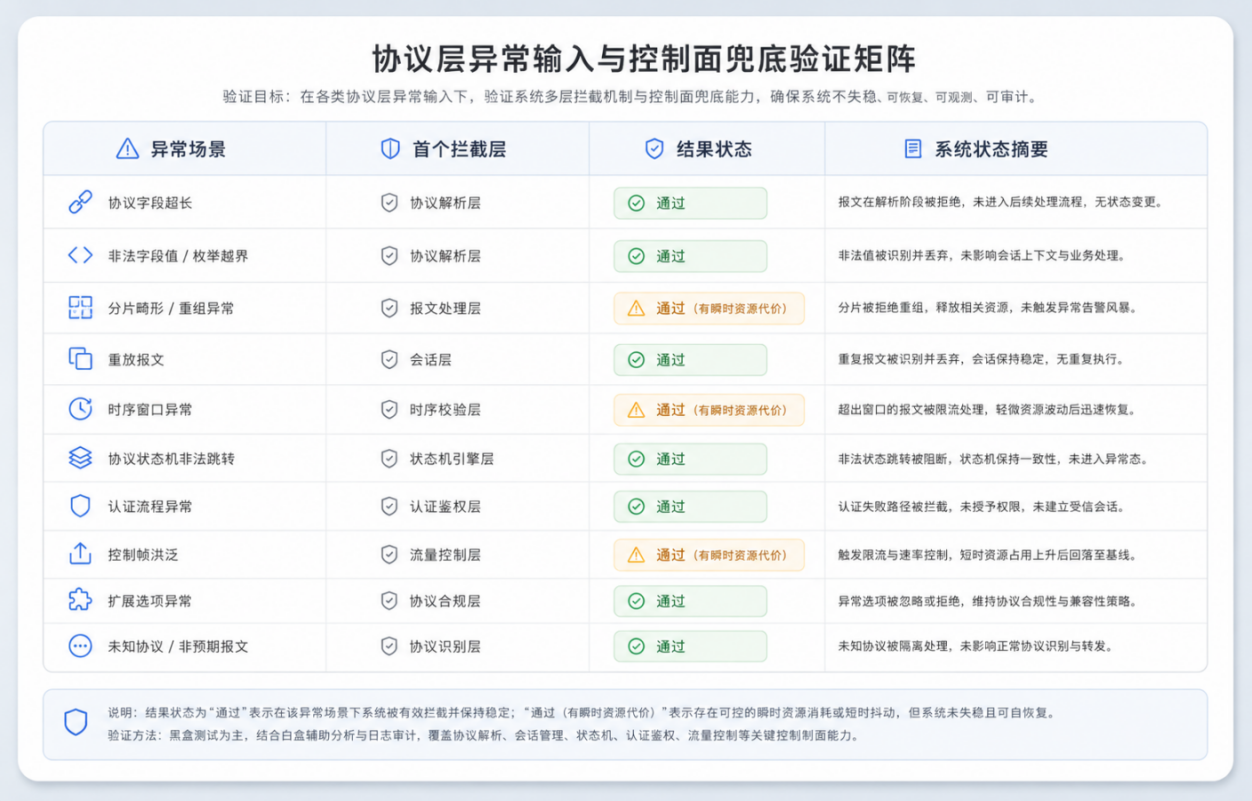
\includegraphics[width=0.92\textwidth]{figures/fig4-2-guard-matrix.png}
\caption{图4-2 医疗动态安全剪枝路径与 DenseNet121 明文基线的概率分布与阈值偏移对比。}
\end{figure}

同口径服务器复核表明，医疗动态安全剪枝链路在 full-val CPU runtime-pruning reference 口径下的 AUC 为 0.9639。这说明当前动态路径并未失去样本排序能力，影响部署效果的关键问题仍然是决策边界相对固定结构参考发生系统性偏移，因此动态路径单独阈值校准仍是正式部署中的必要步骤。

\section{性能与通信量分析}

医疗交付场景与金融边界压力验证场景的端到端性能与通信量统计结果如图4-3所示。

\reportmissingfigure{4-3}{图4-3 不同场景端到端性能与通信量统计}

\noindent\textit{注：通信量为两方节点之间的双向总字节数，包含协议头与控制报文；所有测试均在同机本地双节点（colocated localhost）2PC 模式下执行。}

为进一步量化算子优化的收益，本作品补充了统一基准下的算子级代理对比，结果如表9所示。

\begin{longtable}{>{\raggedright\arraybackslash}p{0.24\textwidth}>{\raggedright\arraybackslash}p{0.24\textwidth}>{\raggedright\arraybackslash}p{0.24\textwidth}>{\raggedright\arraybackslash}p{0.24\textwidth}}
\caption{表 9 算子级代理基准对比结果}\\
\toprule
\textbf{代理基准对比组} & \textbf{通信比值 （左/右）} & \textbf{时间比值 （左/右）} & \textbf{适用范围说明} \\
\midrule
\endfirsthead
\toprule
\textbf{代理基准对比组} & \textbf{通信比值 （左/右）} & \textbf{时间比值 （左/右）} & \textbf{适用范围说明} \\
\midrule
\endhead
同形状算子代理基准 & 0.149x & 0.528x & 同一模型形状、同一 2PC benchmark harness；主要用于观察算子配置导致的安全开销差异。 \\
异构结构代理基准 & 16.845x & 2.955x & 同一 MPCFormer local 2PC benchmark harness；各 profile 使用各自模型结构参数。这不是 full-val 医学图像 pipeline 通信量。 \\
\bottomrule
\end{longtable}

\noindent\textit{注："同形状算子代理基准" 基于统一 DeiT-S 模型结构测试；"异构结构代理基准" 仅用于说明模型结构差异对性能的影响，不代表医疗端到端链路性能。}

为便于统一表达时延与通信量的来源，本节先用式（4-1）至式（4-2）给出端到端代价的分解形式，再结合当前原型链路的实测结果解释主要瓶颈。

\begin{equation}
T_{\text{total}}=T_{\text{pre}}+T_{\text{guard}}+T_{\text{SPU}}+T_{\text{post}}
\tag{4-1}
\end{equation}

\begin{equation}
V_{\text{total}}=\sum_{r}\left(V_{\text{send}}^{r}+V_{\text{recv}}^{r}\right), \quad \rho_V=\frac{V_{\mathrm{Transshield}}}{V_{\text{ref}}}, \quad \rho_T=\frac{T_{\mathrm{Transshield}}}{T_{\text{ref}}}
\tag{4-2}
\end{equation}

其中，$T_{\text{total}}$ 由前端预处理、服务端控制面快检、SPU 密态执行与结果回传/审计收尾四部分组成；$V_{\text{total}}$ 表示一次完整推理的双向总通信量，$\rho_V$ 与 $\rho_T$ 分别表示相对通信量与相对时延比。

性能证据分为两层：其一是上述端到端双向隐私运行结果，用于说明医疗动态安全剪枝链路与金融压力样本在当前原型中的总时延和总通信量；其二是统一安全基准下的算子级代理对比，用于说明算子替换本身的开销趋势。在固定同一 DeiT-S 形状的代理基准对比中，密捷的安全友好算子将通信压缩到外部基准算子的 0.149 倍，时间压缩到 0.528 倍，说明算子替换本身具有正向收益。另一方面，跨模型结构的异构结构代理基准只能用于说明结构尺度差异会显著放大绝对代价，不能与医疗全量验证链路混写。

当前时延与通信量偏高，主要由三类因素共同造成。第一，动态安全剪枝链路保留了词元剪枝的密态比较、排序与掩码化决策链，相比固定结构安全推理会引入额外的协议轮次。第二，当前运行口径是同机本地双节点（colocated localhost）2PC 原型链路，虽然两方节点位于同一服务器内，但张量交换、线性层通信与 softmax 归一化指数函数相关算子仍构成主要代价来源，不能将 localhost 原型误解为“几乎无通信成本”。第三，当前 Web 演示后端以正确性与边界防护为首要目标，未针对生产级吞吐做异步化、流水化或任务队列改造。因此，本报告只保留已直接落盘的端到端结果与算子级代理证据，不额外给出未经观测的阶段占比、P50/P95 延迟或生产级并发吞吐承诺。

\section{金融边界压力验证结果}

金融边界压力验证场景下的核心指标结果如表 10 所示。需要说明的是，金融域原始输入并非自然图像，而是信用卡欺诈检测任务中的 30 维 PCA 特征。为了复用 DeiT-S 的块嵌入（Patch Embedding）结构，本作品先将一维金融特征通过拟图像空间连续性编码映射为 224×224 灰度图，使输入保留可供视觉 Transformer 利用的局部平滑先验。仓内冻结 bundle 记录表明，早期的 patch-based 与 DCT 编码未形成稳定可用结果，当前边界压力验证对应的是 v3 image-like smooth/contrast encoding。

\begin{longtable}{>{\raggedright\arraybackslash}p{0.32\textwidth}>{\raggedright\arraybackslash}p{0.32\textwidth}>{\raggedright\arraybackslash}p{0.32\textwidth}}
\caption{表 10 金融边界压力验证核心指标}\\
\toprule
\textbf{指标} & \textbf{结果} & \textbf{说明} \\
\midrule
\endfirsthead
\toprule
\textbf{指标} & \textbf{结果} & \textbf{说明} \\
\midrule
\endhead
8 条压力样本逐样本一致性 & 8 / 8 样本差异为 0 & 与明文参考逐样本对齐 \\
部署效率 & 106.16 秒/样本 & 仅作为边界压力验证口径 \\
双向总通信量 & 25.30 GiB & 同配置重测口径 \\
参数规模保留比例 & 68.39\% & 体现低秩压缩收益 \\
\bottomrule
\end{longtable}

金融部分仅承担方法迁移性与极端输入稳定性验证职责，不作为与医疗并列的独立交付场景。其价值在于：在不改变安全运行链基本结构的前提下，验证控制面、动态路由与安全执行语义在另一类高敏感任务中的边界表现，从而证明本作品的工程设计并非只对单一数据分布有效。

\section{协议层异常输入与鲁棒性验证}

鲁棒性验证采用穷举边缘分支矩阵，而不是以单一拦截率概括系统表现。协议层测试覆盖分块传输编码（Transfer-Encoding: chunked）、超大报文长度声明（Content-Length）、boundary 参数混淆、重复字段、畸形分片报文头、空字节注入、非空尾部附加数据、UTF-16 编码结构化元数据、超长结构化元数据以及截断请求体；控制面测试覆盖随机一次性标识（Nonce）并发重放、相同载荷更换 Nonce、同一来源地址并发占满与短窗限频。每个用例均记录首个拦截层、兜底层级、返回处置与资源状态回落摘要，以同时证明拦截有效性与系统可服务性。协议层与控制面鲁棒性验证的整体统计结果如表 11 所示。

\begin{longtable}{>{\raggedright\arraybackslash}p{0.16\textwidth}>{\raggedright\arraybackslash}p{0.16\textwidth}>{\raggedright\arraybackslash}p{0.16\textwidth}>{\raggedright\arraybackslash}p{0.16\textwidth}>{\raggedright\arraybackslash}p{0.16\textwidth}>{\raggedright\arraybackslash}p{0.16\textwidth}}
\caption{表 11 协议层与控制面鲁棒性验证统计}\\
\toprule
\textbf{测试组} & \textbf{用例数} & \textbf{按预期通过} & \textbf{FD/Socket无泄漏} & \textbf{稳态回落用例} & \textbf{证据文件} \\
\midrule
\endfirsthead
\toprule
\textbf{测试组} & \textbf{用例数} & \textbf{按预期通过} & \textbf{FD/Socket无泄漏} & \textbf{稳态回落用例} & \textbf{证据文件} \\
\midrule
\endhead
协议层异常输入 & 13 & 13 / 13 & 13 / 13 & 11 / 13 & 协议异常输入验证记录 \\
控制面守卫 & 4 & 4 / 4 & 4 / 4 & 1 / 4 & 控制面守卫验证记录 \\
合计 & 17 & 17 / 17 & 17 / 17 & 12 / 17 & 汇总 \\
\bottomrule
\end{longtable}

从当前留存结果看，协议层异常输入与控制面守卫共覆盖 17 类黑盒用例，17/17 均返回预期拦截或限制结果；全部用例在采样窗口内均未观察到文件描述符或套接字文件描述符的净增长。与此同时，部分并发与大负载探针会带来瞬时常驻内存抬升，因此本作品将其如实记录为“资源成本存在但句柄未泄漏”，而不是将其包装为零成本防护。

为适配 A4 版面，鲁棒性验证矩阵拆分为两张窄表：前表记录攻击特征与拦截链，后表记录返回处置、资源状态与证据来源；为便于对照阅读，第二张表重复给出“异常场景”列。其中，表示文件描述符数量变化，表示套接字文件描述符数量变化，表示常驻内存变化，表示线程数变化，四项指标均按异常处理后观测值减去基线观测值计算。各类异常场景的攻击特征与系统拦截层级明细如表 12 所示。对应异常场景的系统返回处置、资源状态与证据来源明细如表13所示

\begin{longtable}{>{\raggedright\arraybackslash}p{0.24\textwidth}>{\raggedright\arraybackslash}p{0.24\textwidth}>{\raggedright\arraybackslash}p{0.24\textwidth}>{\raggedright\arraybackslash}p{0.24\textwidth}}
\caption{表 12 异常场景攻击特征与拦截层级明细（上）}\\
\toprule
\textbf{异常场景} & \textbf{攻击载荷特征} & \textbf{首个拦截层级} & \textbf{兜底层级} \\
\midrule
\endfirsthead
\toprule
\textbf{异常场景} & \textbf{攻击载荷特征} & \textbf{首个拦截层级} & \textbf{兜底层级} \\
\midrule
\endhead
Chunked 编码绕过 & Transfer-Encoding: chunked，绕过 Content-Length & HTTP 请求体入口门 & 不适用 \\
超大 Content-Length & 声明体积超过 5 MiB，验证 413 + 强制阻断 & Content-Length 头部上限门 & TCP 强制阻断兜底 \\
重复字段名 & 重复注入 multipart 字段，诱导字段集歧义 & raw multipart 预检 & MIME 结构校验 \\
Boundary 扇出 & 构造过多分片，放大 MIME 解析树 & raw multipart 预检 & MIME 结构校验 \\
嵌套 multipart & 把 share part 伪装成 multipart/mixed & raw multipart 预检 & MIME 结构校验 \\
超长 JSON & client\_quality\_summary 超过 JSON 字节门 & JSON 字节长度门 & 严格 JSON 解码钩子 \\
字段集漂移 & 追加未声明字段，验证精确字段集约束 & raw multipart 预检 & 精确字段集门 \\
Boundary 参数混淆 & boundary 带空白与引号变体 & Content-Type boundary 解析 & raw multipart 预检 \\
畸形 Part Header & 缺失合法头格式，验证 header parser & multipart header 解析 & MIME 结构校验 \\
Header 空字节注入 & 在 part header 中注入 NUL / 控制字符 & multipart header 解析 & MIME 结构校验 \\
非空 Epilogue & closing boundary 后继续追加垃圾字节 & raw multipart 预检 & MIME 结构校验 \\
异常 JSON 字符集 & UTF-16LE 编码结构化元数据，验证严格 UTF-8 约束 & strict UTF-8 JSON 解码 & JSON 数值钩子 \\
截断请求体 & 提前断流，验证 streaming body reader & 流式 body 读取器 & 不适用 \\
重复 Nonce 并发重放 & 同 nonce 并发多发，验证幂等与重放防护 & Nonce 重放缓存门 & payload 指纹去重门 \\
同载荷换 Nonce & 相同 share 指纹 + 新 nonce，验证 payload 去重 & 载荷重放缓存门 & IP inflight 配额门 \\
同 IP 并发占满 & 单一来源地址并发冲击已通过前置校验的执行配额 & 单 IP inflight 守卫 & 全局 inflight 守卫 \\
短窗限频 & 同 IP 短时间空载请求探测限流门 & IP 滑动窗口限频 & 不适用 \\
\bottomrule
\end{longtable}

\begin{longtable}{>{\raggedright\arraybackslash}p{0.24\textwidth}>{\raggedright\arraybackslash}p{0.24\textwidth}>{\raggedright\arraybackslash}p{0.24\textwidth}>{\raggedright\arraybackslash}p{0.24\textwidth}}
\caption{表 13 异常场景返回处置与系统状态明细（下）}\\
\toprule
\textbf{异常场景} & \textbf{返回/处置} & \textbf{系统状态} & \textbf{证据来源} \\
\midrule
\endfirsthead
\toprule
\textbf{异常场景} & \textbf{返回/处置} & \textbf{系统状态} & \textbf{证据来源} \\
\midrule
\endhead
Chunked 编码绕过 & HTTP 400 / transfer\_encoding\_not\_supported & ；；KiB； & 协议异常输入验证记录 / A1 \\
超大 Content-Length & HTTP 413 / payload\_too\_large & ；；KiB； & 协议异常输入验证记录 / A2 \\
重复字段名 & HTTP 400 / malformed\_multipart\_precheck\_failed & ；；KiB； & 协议异常输入验证记录 / A3 \\
Boundary 扇出 & HTTP 400 / malformed\_multipart\_precheck\_failed & ；；KiB； & 协议异常输入验证记录 / A4 \\
嵌套 multipart & HTTP 400 / malformed\_multipart\_precheck\_failed & ；；KiB； & 协议异常输入验证记录 / A5 \\
超长 JSON & HTTP 400 / invalid\_control\_plane\_payload & ；；KiB； & 协议异常输入验证记录 / A6 \\
字段集漂移 & HTTP 400 / malformed\_multipart\_precheck\_failed & ；；KiB； & 协议异常输入验证记录 / A7 \\
Boundary 参数混淆 & HTTP 400 / malformed\_multipart\_precheck\_failed & ；；KiB； & 协议异常输入验证记录 / A8 \\
畸形 Part Header & HTTP 400 / malformed\_multipart\_precheck\_failed & ；；KiB； & 协议异常输入验证记录 / A9 \\
Header 空字节注入 & HTTP 400 / malformed\_multipart\_precheck\_failed & ；；KiB； & 协议异常输入验证记录 / A10 \\
非空 Epilogue & HTTP 400 / malformed\_multipart\_precheck\_failed & ；；KiB； & 协议异常输入验证记录 / A11 \\
异常 JSON 字符集 & HTTP 400 / invalid\_control\_plane\_payload & ；；KiB； & 协议异常输入验证记录 / A12 \\
截断请求体 & HTTP 400 / truncated\_body & ；；KiB； & 协议异常输入验证记录 / A13 \\
重复 Nonce 并发重放 & duplicate\_nonce×3；200×1 & ；；KiB； & 控制面守卫验证记录 / G1 \\
同载荷换 Nonce & 首发 200；复发 duplicate\_payload & ；；KiB； & 控制面守卫验证记录 / G2 \\
同 IP 并发占满 & 200×2；busy\_retry\_later×2 & ；；KiB； & 控制面守卫验证记录 / G3 \\
短窗限频 & invalid\_content\_length×6；rate\_limited\_ip×2 & ；；KiB； & 控制面守卫验证记录 / G4 \\
\bottomrule
\end{longtable}

\noindent\textit{注：系统状态指标 ΔFD、ΔSock、ΔRSS、ΔThr 均为异常处理完成后 10 秒的观测值与基线值的差值；所有证据文件均已留存于仓内 tools/evidence 目录。}

\reportmissingfigure{4-4}{图4-4 协议层异常输入与控制面兜底验证矩阵：同时显示首个拦截层级与文件描述符、套接字及常驻内存回落摘要。}

资源状态采用可观测代理指标描述，而不作无法直接证明的绝对化承诺。本文将“系统仍可服务”限定为：请求结束后 inflight 占用计数回落，文件描述符数量与套接字文件描述符数量回到基线附近，未观察到连接句柄持续泄漏；常驻内存在部分已通过前置校验的压力用例中出现瞬时抬升，但重复异常注入测试后未观察到单调持续增长，因此仅将其表述为原型阶段的瞬时资源成本，而不宣称所有指标完全归零。

\section{结果分析}

综合上述结果可以得到三个结论。第一，本作品动态安全剪枝链路的主要收益并非体现在超越强明文参考，而是体现在双向隐私约束下保留了可部署的动态剪枝能力，并通过阈值校准把全量验证集精度恢复到 92.7481\%。第二，算子级代理对比说明安全友好算子本身具有明显的通信与时间收益，但结构尺度差异仍然是当前端到端时延偏高的关键原因。第三，协议层异常输入与控制面探针在当前实现下能够被前置阻断，且未观察到文件描述符或套接字句柄的持续泄漏，这为系统的原型级可服务性提供了必要的证据支撑。

若将本作品放回现有私有 Transformer 推理研究中理解，可以发现本作品当前结果更接近“在医疗视觉任务中建立动态剪枝双向隐私闭环”的工程验证，而非单纯追求固定结构模型的最低时延。Iron[18]、BOLT[19]、NEXUS[20] 与 CipherPrune[21] 的公开结果表明，协议级优化、非交互执行或密态渐进剪枝都可能显著改善特定模型的绝对效率；而本作品当前结果说明，在浏览器端本地分片、服务端权威快检和两方安全执行同时成立的前提下，动态剪枝边界保留本身就是一个独立目标。因此，本作品的评价重点应同时包含“闭环是否成立”和“效率是否仍可继续优化”两个层次，而不是只以单一时延指标作判断。

结果解释需要区分三类比较口径。第一类是同仓动态链路与静态安全基线的比较，用于判断动态剪枝安全化改写是否带来部署收益；第二类是同数据集强明文参考，用于说明当前安全化改写距离普通明文模型还有多大差距；第三类是外部私有推理系统或论文结果，用于定位技术路线，但不能直接与本作品端到端 Web 控制面、双向隐私和本地双节点 SPU 原型混作数值对比。按这一口径理解，当前实验结果的核心结论是：动态剪枝在安全执行域内具有可保留的判别价值，同时端到端效率仍有明显工程优化空间。

\section{消融实验与必要性验证}

为验证各关键设计的必要性，本文进一步从模型路径与控制面两条主线开展消融分析。图4-5给出了医疗动态安全剪枝链路、去掉动态剪枝后的静态安全基线以及原始明文参考基线的同口径对照结果。可以看到，在524张全量验证集样本上，医疗动态安全剪枝链路的阈值精度达到92.7481\%，高于去掉动态剪枝后的静态安全基线89.6947\%，提升3.0534个百分点；AUC由0.9539提升至0.9639，增幅为0.0100。与此同时，医疗动态安全剪枝链路的argmax精度并未高于静态安全基线，说明动态剪枝安全化改写的主要价值不在于未校准条件下的直接分类，而在于部署口径下更稳定、更可校准的判别边界。

进一步地，与原始明文参考基线相比，医疗动态安全剪枝链路的阈值精度提升17.3664个百分点，表明本作品并非仅在外层增加安全计算壳，而是在动态剪枝边界、固定图安全语义和部署后阈值校准之间形成了协同增益。

在控制面方面，现有协议层异常输入与控制面探针共覆盖17类黑盒用例，17/17均返回预期拦截或限制结果；同时审计日志表明，重复载荷会被重放守卫以duplicate\_payload阻断，正常请求则被记录为quality\_status=pass。上述结果说明，服务端权威快检、重放防护、并发门控和审计链并非展示性附件，而是保证异常输入止于SPU之前、非法重放止于控制面边界、运行状态可复核的必要组成部分。

\reportmissingfigure{4-5}{图4-5 动态剪枝消融结果（524张验证集，同口径）}

其中，医疗动态安全剪枝链路相较静态安全基线的阈值精度提升3.0534个百分点，AUC提升0.0100；相较原始明文参考基线的阈值精度提升17.3664个百分点。
